\documentclass{article}
\usepackage{tikz}
\usepackage{xcolor}

\definecolor{myblue}{RGB}{40,110,160}
\definecolor{bggray}{RGB}{245,245,245}
\definecolor{gridgray}{RGB}{180,180,180}

\begin{document}

\begin{center}
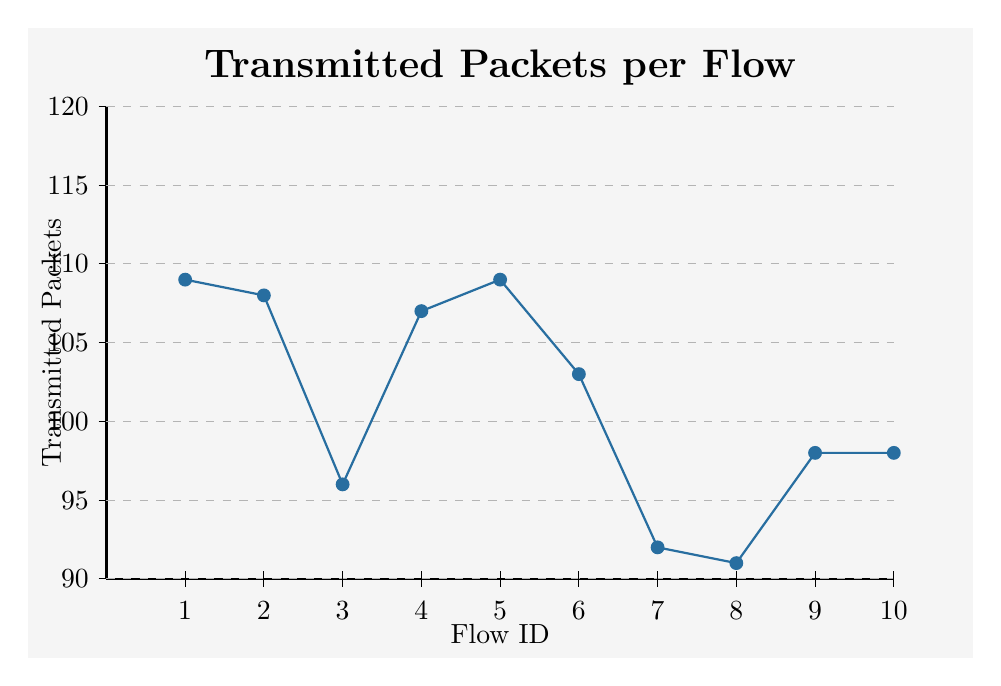
\begin{tikzpicture}

% Background
\fill[bggray] (0,0) rectangle (12,8);

% Axes
\draw[thick] (1,1) -- (1,7);
\draw[thick] (1,1) -- (11,1);

% Title
\node[font=\Large\bfseries] at (6,7.5) {Transmitted Packets per Flow};

% Labels
\node[rotate=90] at (0.3,4) {Transmitted Packets};
\node at (6,0.3) {Flow ID};

% Y-axis ticks (range ~90 to 110)
\foreach \y/\val in {
1/90,
2/95,
3/100,
4/105,
5/110,
6/115,
7/120
}{
\draw (0.9,\y) -- (1.1,\y);
\node[left] at (0.9,\y) {\val};
\draw[dashed, gridgray] (1,\y) -- (11,\y);
}

% X-axis ticks
\foreach \x in {1,...,10}{
\draw (\x+1,0.9) -- (\x+1,1.1);
\node at (\x+1,0.6) {\x};
}

% Scale factor
\def\scale{0.2}

% Line plot
\draw[thick, myblue]
(2,{1+(109-90)*\scale}) --
(3,{1+(108-90)*\scale}) --
(4,{1+(96-90)*\scale}) --
(5,{1+(107-90)*\scale}) --
(6,{1+(109-90)*\scale}) --
(7,{1+(103-90)*\scale}) --
(8,{1+(92-90)*\scale}) --
(9,{1+(91-90)*\scale}) --
(10,{1+(98-90)*\scale}) --
(11,{1+(98-90)*\scale});

% Markers (circles)
\foreach \x/\y in {
2/109,
3/108,
4/96,
5/107,
6/109,
7/103,
8/92,
9/91,
10/98,
11/98
}{
\fill[myblue] (\x,{1+(\y-90)*\scale}) circle (2.5pt);
}

\end{tikzpicture}
\end{center}

\end{document}